\chapter{Umsetzung eines Verteilen Transaktionalen Systems mit dem Actor Model} 
\label{cha:practicalDevelopment}

Während der Umsetzung des Anforderungskataloges aus Abschnitt \ref{sec:Eruierung:technicalRequierements} wurde versucht das erarbeitete Wissen aus den theoretischen Kapitel praktisch anzuwenden. Die implementierte Architektur des Flugbuchungssystem legt seinen Schwerpunkt auf die Verteilung des gesamten Systems. Mit der Nachfolgend vorgestellten Implementierung ist es möglich Anzahl an Instanzen der verschiedenen Komponenten Während des Betriebes beliebig anzupassen. \\
Das folgende Kapitel erklärt den Aufbau der praktischen Anwendung. Nach der Einführung des verwendeten Frameworks um mit dem Actor Model arbeiten zu können, wird zuerst der Komponentenorientierte Aufbau der Implementierung vorgestellt. Anschließend wird auf die Implementierung der Abfrage und Befehlverarbeitung eingegangen, welche auf die starke Orientierung auf Verteilung angepasst ist. Nachfolgend wird die Implementierung der Garantierten Nachrichtenzustellung aus Abschnitt \ref{sec:actor:patterns:guaranteedDelivery} vorgestellt. Abschließend wird das Kapitel die Testapplikation vorstellen mit welcher die verteilte Anwendung geprüft wurde sowie auf die während der Entwicklung verwendete Environment Umgebung einehen.

\section{Einführung in das \textit{Akka.net} Framework}
Das Framework \textit{Akka} stellt das Actor-Model für \textit{Java} und \textit{Scala} Entwickler zur verfügung. Bei Entwickler dieser Sprachen konnte sich das Framework, und somit auch das Actor-Model einen guten Namen machen. Für \textit{.Net} Entwickler mit den Sprachen \textit{C\#} und \textit{F\#} wurde das Projekt mit Hilfe der OpenSource Community unter dem Name \textit{Akka.Net} für die \textit{.Net} Plattform portiert. Somit sind die funktionalität und der Aufbau der Frameworks zwischen \textit{Akka} und \textit{Akka.net} identisch, wenngleich auch die Implementierung, aufgrund der Sprach und Laufzeitunterschiede zwischen der \textit{Java Virtual Machine (JVM)} und der \textit{Common Language Runtime (CLR)}, siehe hierzu \cite{JvmVsClrsinger2003jvm}, unterschiedlich ist. \\
Die Implementierung der hier beschriebenen Anwendung erfolgt für die \textit{CLR}, und somit mit Hilfe des Frameworks \textit{Akka.Net}. 

\subsection{Ein Actor in \textit{Akka.Net}}
Wie bereits erwähnt wird eine Anwendung auf Basis von \textit{Akka.Net} mit der Objektorientierten Sprache \textit{C\#} geschrieben. Somit werden auch Actors als Klassen repräsentiert. In \textit{Akka.Net} gibt dafür Basisklassen welche die Funktionalität eines Actors, wie die Nachrichtenübermittelung oder das Verhalten auf empfangene Nachrichten, beinhalten. Die Actor Klasse selbst bietet jedoch für andere Klassen keine eigenen Methoden zur verfügung. Somit ist der Zugriff von Außen, wie in Abschnitt \ref{actor:requirements:shareNothing} beschrieben, nicht möglich. \\

\subsubsection{Nachrichten}\label{subsec:implementation:akkaMessaging}
Da ein Actor selbst keine Methoden anbietet erfolgt die Interaktion mit der Umwelt des Actors über Nachrichten. Dies wird in \textit{Akka.Net} durch Objekte sichergestellt. Eine Nachricht selbst muss in \textit{Akka.Net} keine bestimmte Struktur aufweisen, kann somit von jedem beliebigen Datentyp sein. Um jedoch die zustellung von Nachrichten über verschiedene Hosts zu gewähreisten, siehe dazu Abschnitt \ref{subsec:implementation:ApplicationDistribution}, sollte eine Nachricht serialisierebar sein. Dies ist jedoch für Nachrichten welche innerhalb einer Laufzeitinstanz übertragen werden nicht relevant. \\
Um nun eine Nachricht an einen Actor zu senden, wird die Referenz des Actors , siehe dazu Abschnitt \ref{subsec:implementation:ApplicationDistribution}, benötigt an welche die Nachricht gerichtet ist. Auf diese Referenz, welche ja selbst eine Instanz vom Typ \textit{ActorRef} ist, können nun für die übermittlung der Nachricht die Methoden \textit{Tell} oder \textit{Ask} aufgerufen werden.
\begin{description}
    \item[Tell] Möchte man eine Nachricht an einen Actor senden ohne auf dessen Antwort zu warten, so wie es das theoretische \textit{Actor Model} auch vorsieht, sollte die Methode \textit{Tell} verwendet werden. Die Methode selbst blockiert nicht, und die Nachricht wird in einem Thread an den Actor zugestellt. 
    \item[Ask] Die Methode \textit{Ask} blockiert den aktuellen Thread, bis eine Antwort auf die gesendet Nachricht zugestellt wird. Somit gleicht \textit{Ask} einem gewöhnlichen Methodenaufruf. Diese Variante verletzt jedoch die zweite Bedingung eines Actors aus Abschnitt \ref{actor:requirements:AsynchronCommunication}, welche besagt das die Kommunikation zwischen Actoren frei von Wartemechanismen sein sollte. Deshalb ist diese Variante für die zustellung von Nachrichten nur im Ausnahmefall zu empfehlen.  
\end{description}
Nachrichten welche über die Actor Referenz mit den eben beschriebenen Methoden zugestellt worden sind, werden in die Mailbox des Empfängers eingereiht. Enthält der Empfänger ein Verhalten für diesen Typ der Nachricht, so wird, sobald die Nachricht vom Actor aus der Mailbox genommen wird, diese Abgearbeitet. Enthält der Actor für diese Nachricht jedoch kein Verhalten, so wird die Nachricht verworfen, der Sender der Nachricht bekommt dies jedoch nicht mit. 

\begin{lstlisting}[caption=Versenden einer Nachricht an einen anderen Actor, label=code:actor:TellMethod]
    targetActorRef.Tell(new SpecificMessage());
\end{lstlisting}

\begin{lstlisting}[caption=Hier wird für den Actor \textit{MyTargetActor} das Verhalten für eine Einkommende Nachricht vom Typ \textit{SpecificMessage} festgellegt., label=lst:test]
    public sealed class MyTargetActor : ReceiveActor {
        public MyTargetActor() {
            Become<SpecificMessage>(x => {
                Console.Log("Nachricht von Typ SpecificMessage empfangen");
                //implement logic for handling SpecificMessage
            })
        }
    }    
\end{lstlisting}

\subsubsection{Erstellung von Actors}
\label{subsec:implementation:actorCreation}
Die Erstellung einer Instanz eines Actors erfolgt nicht über das Schlüsselwort \textit{new}, sondern wird vom Framework selbst übernommen. Dazu werden dem Framework alle Informationen zur verfügung gestellt welche es benötigt um den Actor zu erstellen, das beinhaltet beispielsweise den Typ des Actors, dessen Abängigkeiten sowie gegebenenfalls der Ort an welcher der Actor erstellt werden soll. Anschließend bekommt der aufrufer der erzeugung eine Referenz, die sogenannte \textit{ActorRef}, welche dazu dient mit dem erstellten Actor, über die Methoden aus Abschnitt \ref{subsec:implementation:akkaMessaging} zu kommunizieren. Eine direkte Referenz auf den Actor selbst wird nicht zur verfügung gestellt. \\
Durch die Verwendung einer eigenen, Framework basiertem Referenz anstatt einer direkten Referenz auf den Actor, können Actors ortsungebunden instanziiert werden ohne das der Anwender des Actors dies im Code beachten muss. Die Verwendung eines Actors unterscheidet sich somit nicht davon ob er sich in der gleichen Laufzeitumgebung befindet oder ob er sich auf einem örtlich getrennten System befindet und die Verbindung zu diesem Actor über ein Netzwerk hergestellt wird. Die Informationen wo die einzelnen Actors wirklich instanziert werden, wird über eine Konfigurations Datei gesteuert. Somit kann das Verhalten des Systems einfach geändert werden und die Verteilung der gesamten Applikation wird erleichtert.

\section{Service Architektur}
Um dasFlugbuchungssystem zu realisieren wurde auf eine Komponenten und Serviceorientierte Architektur geachtet. Dazu wurden die Anforderungen selbst in einzelne Kategorien unterteilt und daraus verschiedene Komponenten abgeleitet. \\
Einerseits besteht die Applikation aus einer Schnittstelle zu den Endbenutzer welche über \textit{HTTP} Aufrufe Anfragen an das System durchführen können. Die Anfragen selbst können entweder in Abfragen oder in Kommandos unterteilt werden. Somit ist eine weitere Komponente auf Abfragen (\textit{Queries}) spezialisiert und eine weitere Komponente behandelt Kommandos welche Daten im System verändern können. Alle Prozessebezogenen Inhalte werden in der Komponente \textit{Domain Model} behandelt. In dieser befindet sich die Logik des Flugbuchungssystem welche auch für die einhaltung der Datenkonsistenz zuständig ist. \\
Abschließend wird noch eine Komponente benötigt welche diese Komponenten miteinander in Verbindung bringt. Ableitend aus der \textit{Akka.Net} Community wird diese \textit{Lighthouse} genannt. Somit existieren in der \textit{TyrolSky} Anwendung folgende Komponenten:
\begin{itemize}
    \item API
    \item Query-Service
    \item Command-Service
    \item Domain-Service
    \item Lighthouse
\end{itemize}
Von jeder dieser Komponenten kann es zur Laufzeit mehrere Instanzen davon geben. 
Jeder dieser Komponenten kann mehrfach Instanziiert werden und somit die Last verteilen. Für eine korrekt Arbeitendes System ist es erforderlich das von jeder Komponente mindestens eine Instanz am System teilnimmt. Jedoch können teile des System auch funktionieren wenn nicht alle Komponenten verfügbar sind. So ist es beispielsweise möglich das Abfragen auf das System durchführbar sind obwohl keine Instanz von \textit{Domain Service} oder \textit{Command-Service} verfügbar sind. Jedoch können dann Befehle wie Tickets kaufen nicht durchgeführt werden und würden zu einem Fehler beim Benutzer führen. \\
Nun wird auf die genauere Funktionsweise und zuständigkeiten der einzelnen Komponenten eingegangen.

\subsection{\textit{Lighthouse}}
\label{subsec:implementation:lighthouse}
Dieser Service ist der einfachste und beinhaltet keine Logik welche speziell für die \textit{TyrolSky} Anwendung gedacht ist. Die für die vorliegende Anwendung eingesetzte  Version ist eine Abwandlung des öffentlich zugänglichen Basiscodes einer Lighthouse, siehe hierzu \cite{lighthouse}. \\
Die Komponente fungiert, wie ihr Name schon suggeriert, als Orientierungshilfe für neue Instanzen welche am gesamten System teilnehmen möchten. Diese Melden sich bei einem oder mehreren Laufenden Instanzen von \textit{Lighthouse} an und bekommen somit die Informationen von anderen Komponenten welche sich bereits im System befinden mit. Dieser Prozess wird in Abschnitt \ref{subsec:implementation:gossip} genauer beschrieben.

\subsection{\textit{API}-Schnittstelle}
\label{subsec:implementation:apiComponente}
Anfragen von Endbenutzern werden über eine \textit{REST} Schnittstelle mittels \textit{HTTP} an das System übertragen. Diese Anfragen werden von der Komponente \textit{API} angenommen. Anschließend wird von dieser die Anfrage geprüft, und anschließend an eine verfügbare \textit{Query} oder \textit{Command} Komponente weitergeleitet. \\
Für jede ankommende Anfrage, wird ein eigener Actor gestartet welche ausschließlich für diese konkrete Anfrage zuständig ist. Der Actor wartet auf eine Antwort von der Angefragten \textit{CQRS}-Komponente und beendet nach Abschließend die bestehende \textit{HTTP}-Verbindung zum Benutzer mit dem Entsprechenden Ergebnis. Wird von der Anfragten Komponente innherhalb eines Zeitfensters keine Antwort geliefert wird die Anfrage zum Benutzer mit einem Fehler abgebrochen. \\
In der Grafik \ref{fig:implementation:apiActorModel} ist der Aufbau des Actor Models innerhalb der API Komponente ersichtlich. Darauf ist auch zu sehen das die API Komponente selbst über keine Komplexen Aufbau verfügt und die Actoren darin als Actor Rezeptionisten wie in Kapitel \ref{actor:actorSystem} fungieren und somit eine Schnittstelle zum eigentlichen Actor System selbst herstellen. \\
Das Verwenden von einem separaten Rezeptionisten pro Benutzeranfrage ermöglicht es, die weitere Behandlung im dahinterliegenden Actorsystem an unterschiedliche Komponenteninstanzen zu verteilen. Dadurch können gleiche Anfragen an die selbe API Instanz von unterschiedlichen Instanzen der zuständigen Komponente abgearbeitet werden. 
\begin{figure}
    \centering
    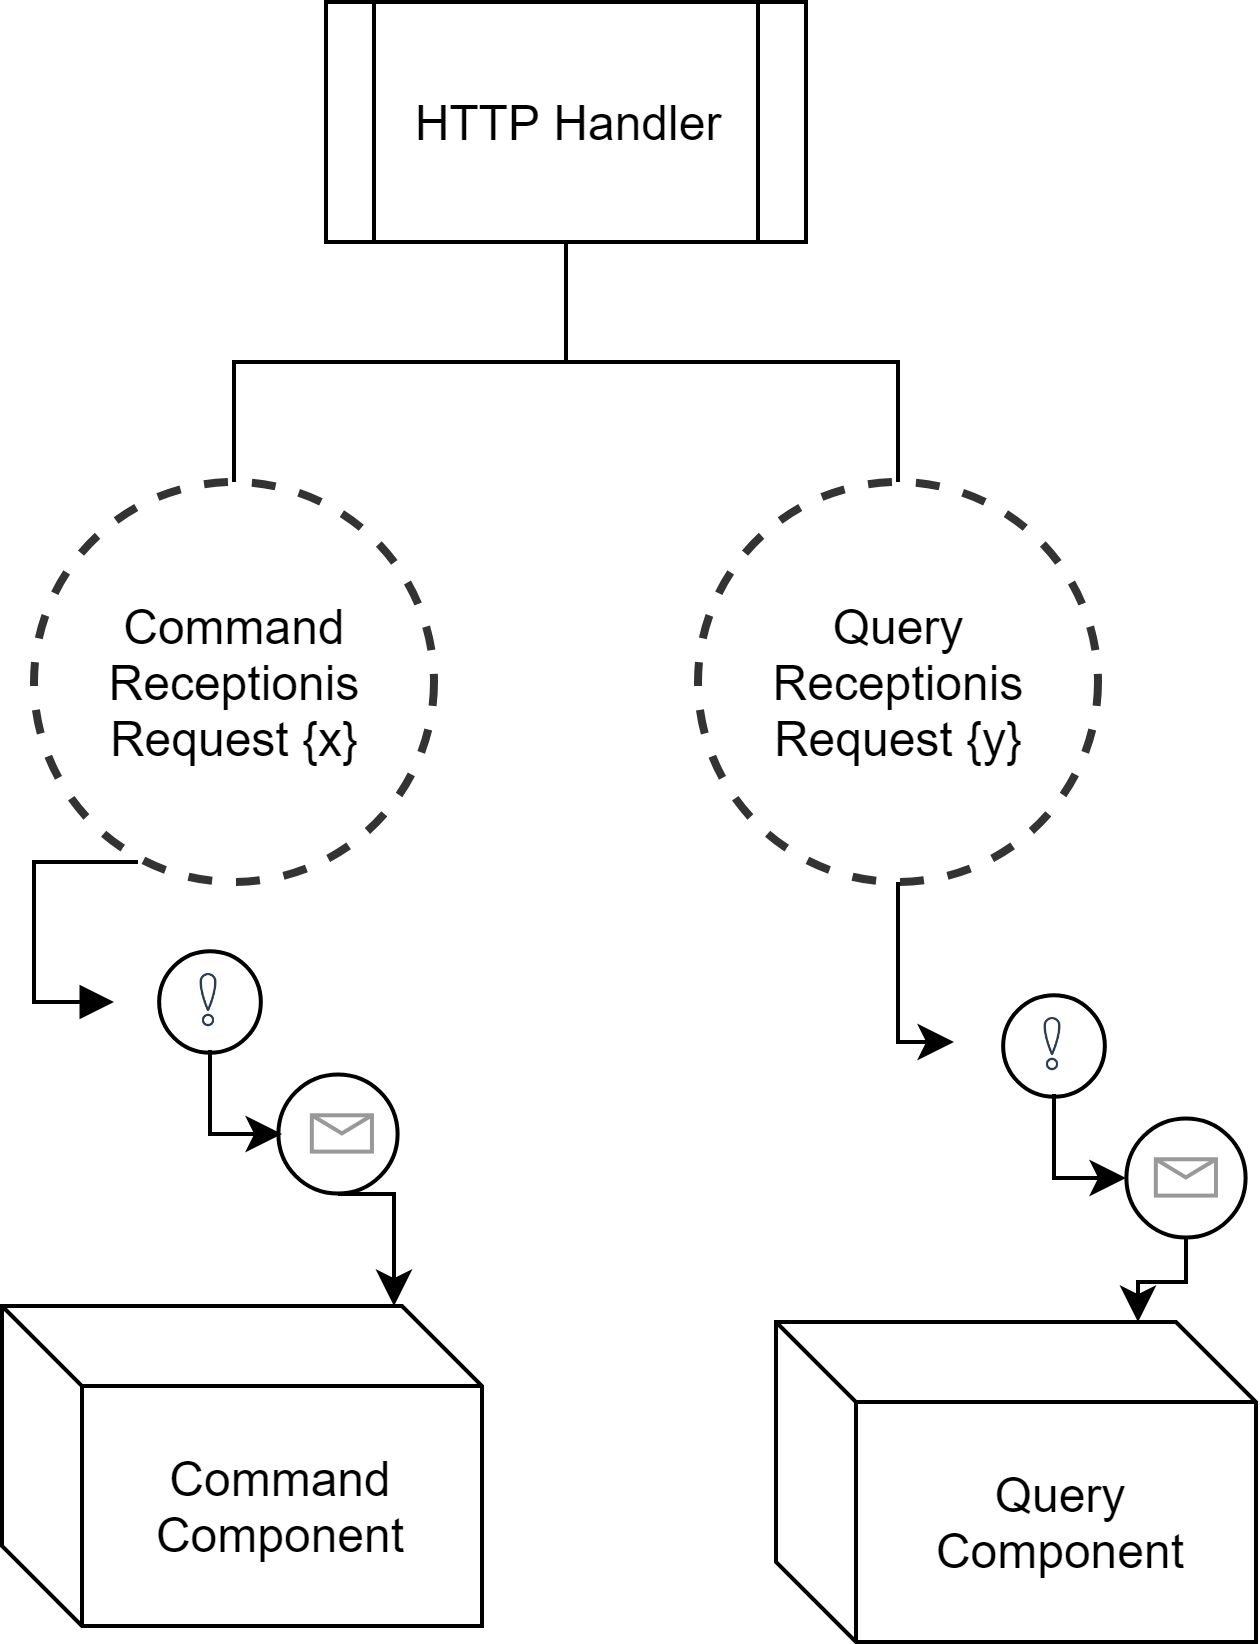
\includegraphics[width=0.5\linewidth]{gfx/implementation/apiActorModel}
    \caption{Actor Ansicht der API Komponente}
    \label{fig:implementation:apiActorModel}
\end{figure} 

\subsection{Query-Service}
Die Anwendung separiert wie bereits erwähnt Abfragen und Befehle nach dem \textit{CQRS} Prinzip auf welches in Kapitel \ref{sub:transaction:cqrs} eingegangen wird. Die Abfrage Seite wird in der Implementierung der \textit{TyrolSky} Anwendung in einer eigenen Komponente realisiert. \\
Um Anfrage bearbeiten zu können welche eine Abfrage an das System stellen, überwacht die Komponente relevante Events welche im Event Sourcing, siehe dazu \ref{subsec:implementation:eventSouring}, aufgetreten sind. \\
Für jeden Typ von Abfrage wird dazu ein vorbereitetes Ergebnis bereit gehalten. Wird ein relevantes Event im Event Sourcing gefunden, so wird das Ergebnis mit den neuen Eventdaten aktualisiert. Dadurch können bei eintreffenden Anfragen diese, durch das bereits vorbereitete Ergebnis, ohne weitere Abfragen an ein Datenbanksystem oder ähnliches, abgearbeitet werden. Jedoch sind die Resultate einer Abfrage nicht garantiert aktuell. Wird ein bereits eingetretendes Event zu spät in das vorbereitete Ergebnis miteingerechnet, bekommt der Anfragende das Ergebnis zurückgeliefert, welches vor dem Event gegolten hat. Deshalb wird diese Komponente nur für Anfragen von Benutzern verwendet und keine applikatorischen Entscheidungen darauf aufgebaut.

\subsubsection{Aufbereitung von Resultaten}
Tretten neue Events auf, so wird die Resultatsliste aktualisiert. Wird eine neue Instanz der \textit{Query} Komponente gestartet, so muss diese zuerst alle im System befindlichen Events abarbeiten um ein aktuelles Ergebnis ausliefern zu können. Da dies bei einer vielzahl von Events Zeit und Ressourcen benötigt, werden aufbereitete Resultate selbst wieder abgespeichert. Dies passiert sporadisch nach einer bestimmten Menge an bearbeitenden Events. Wird das System neugestartet, kann auf das letzte abgespeicherte Resultat zurückgegriffen werden, und anschließend auf diesem weitergearbeitet werden. \\
Die Speicherung von Ergebnis führt jedoch zu Problemen wenn man die Verteilung der Komponente beachtet. Da jede Instanz seine eigenen Ergebnisse vorbereitet müssen diese auch eigenständig gespeichert werden. Ansonsten ergeben sich beim Schreiben als auch beim Lesen konflikte zwischen den einzelnen Instanzen. Um dies zu umgehen wird entweder pro Instanz eine eigene permanente Persistierung, wie beispielsweise eine Datenbank, eingerichtet. Jedoch erhöht dies den Wartungsaufwand der Komponente da für jede Instanz eine eigene Datenbank gehalten werden muss. \\

Eine weitere Möglichkeit ist die Persistierung der Ergebnis pro Komponente in einer globalen Datenbank, wobei jeder Erzeuger von Ergebnissen seine Resultate mit einer Identifikation abspeichert. Dafür ist es jedoch erforderlich das Erzeuger von Ergebnissen eine eindeutige Identifikation besitzen. Dafür wurde ein globaler Namensservice eingerichtet, der im gesamten verteilten System eindeutige Namen vergibt. Meldet sich eine Komponente vom System ab, werden alle Namen, welche an diese Komponente vergeben wurden, wieder freigegeben. Meldet sich eine Komponente wieder beim System an, so bekommt diese die wieder freigegebenen Identifikationen. Diese kann somit mit den Ergebnissen der vorherigen Komponente, welche sich nicht  mehr im System befindet, weiterarbeiten. Für die Umsetzung des globalen Namensservice wurde auf das Pattern \textit{Cluster Singelton}, welches in Abschnitt \ref{subsec:implementation:singeltons} erklärt wird. \\
Durch die Verwendung einer globalen Datenbank, sowie auf daszurückgreifen eines globalen Namensservice ist während dem Betrieb der Anwendung der Wartungsaufwand auf ein minimum beschränkt. Weiters kann durch diese Variante sichergestellt werden, das bei bei einem neustart des Systems die Instanzen mit bereits zuvor erarbeiteten Resultaten weiterarbeiten können. 

\subsubsection{Implementierte Abfrage}
In der umgesetzten Implementierung werden Abfragen zur verfügung gestellt welche dem Benutzer eine Übersicht über angebotente Flüge sowie den Status von Flugtickets geben. Insgesamt sind drei unterschiedliche Abfragen möglich:

\begin{enumerate}
    \item Status eines Flugtickets Abfragen
    \item Liste alle zur verfügung stehenden Flüge
    \item Passagierliste eines bestimmten Fluges
\end{enumerate}

Für die dritte Abfrage wurde jedoch eine andere Abfragevariante gewählt. Anstatt auf Events zu horchen, wird die Abfrage direkt an die entsprechenden Domaineninstanzen (siehe dazu Abschnitt \ref{subsec:implementation:domainService}) weitergegeben. Dies führt dazu, dass die Abfrage selbst länger dauert, da keine Ergebnisse vorgehalten werden. Jedoch ist die abfrage selbst zeitlich exakter, und der Aufwand in der Entwicklung geringer. \\
Das Beispiel zeigt, dass je nach Anwendungsfall entschieden werden sollte wie die Abfrage von Daten exakt implementiert wird.

\subsubsection{Strukturierung}
Für die abarbeitung einzelner Abfragen wird, ähnlich wie bei der Komponente \textit{API} aus Abschnitt \ref{subsec:implementation:apiComponente}, auch für die realisierung von Abfragen auf die Hilfe von kurzlebige Actoren gesetzt. Diese führen den eigentlichen Abfrageprozess durch, und verwenden dazu die enstprechenden Query Actoren. In Abbildung \ref{fig:implementation:queryActorModel} ist der Aufbau der Query Komponente in Form von Actoren zu sehen. 
\begin{figure}
    \centering
    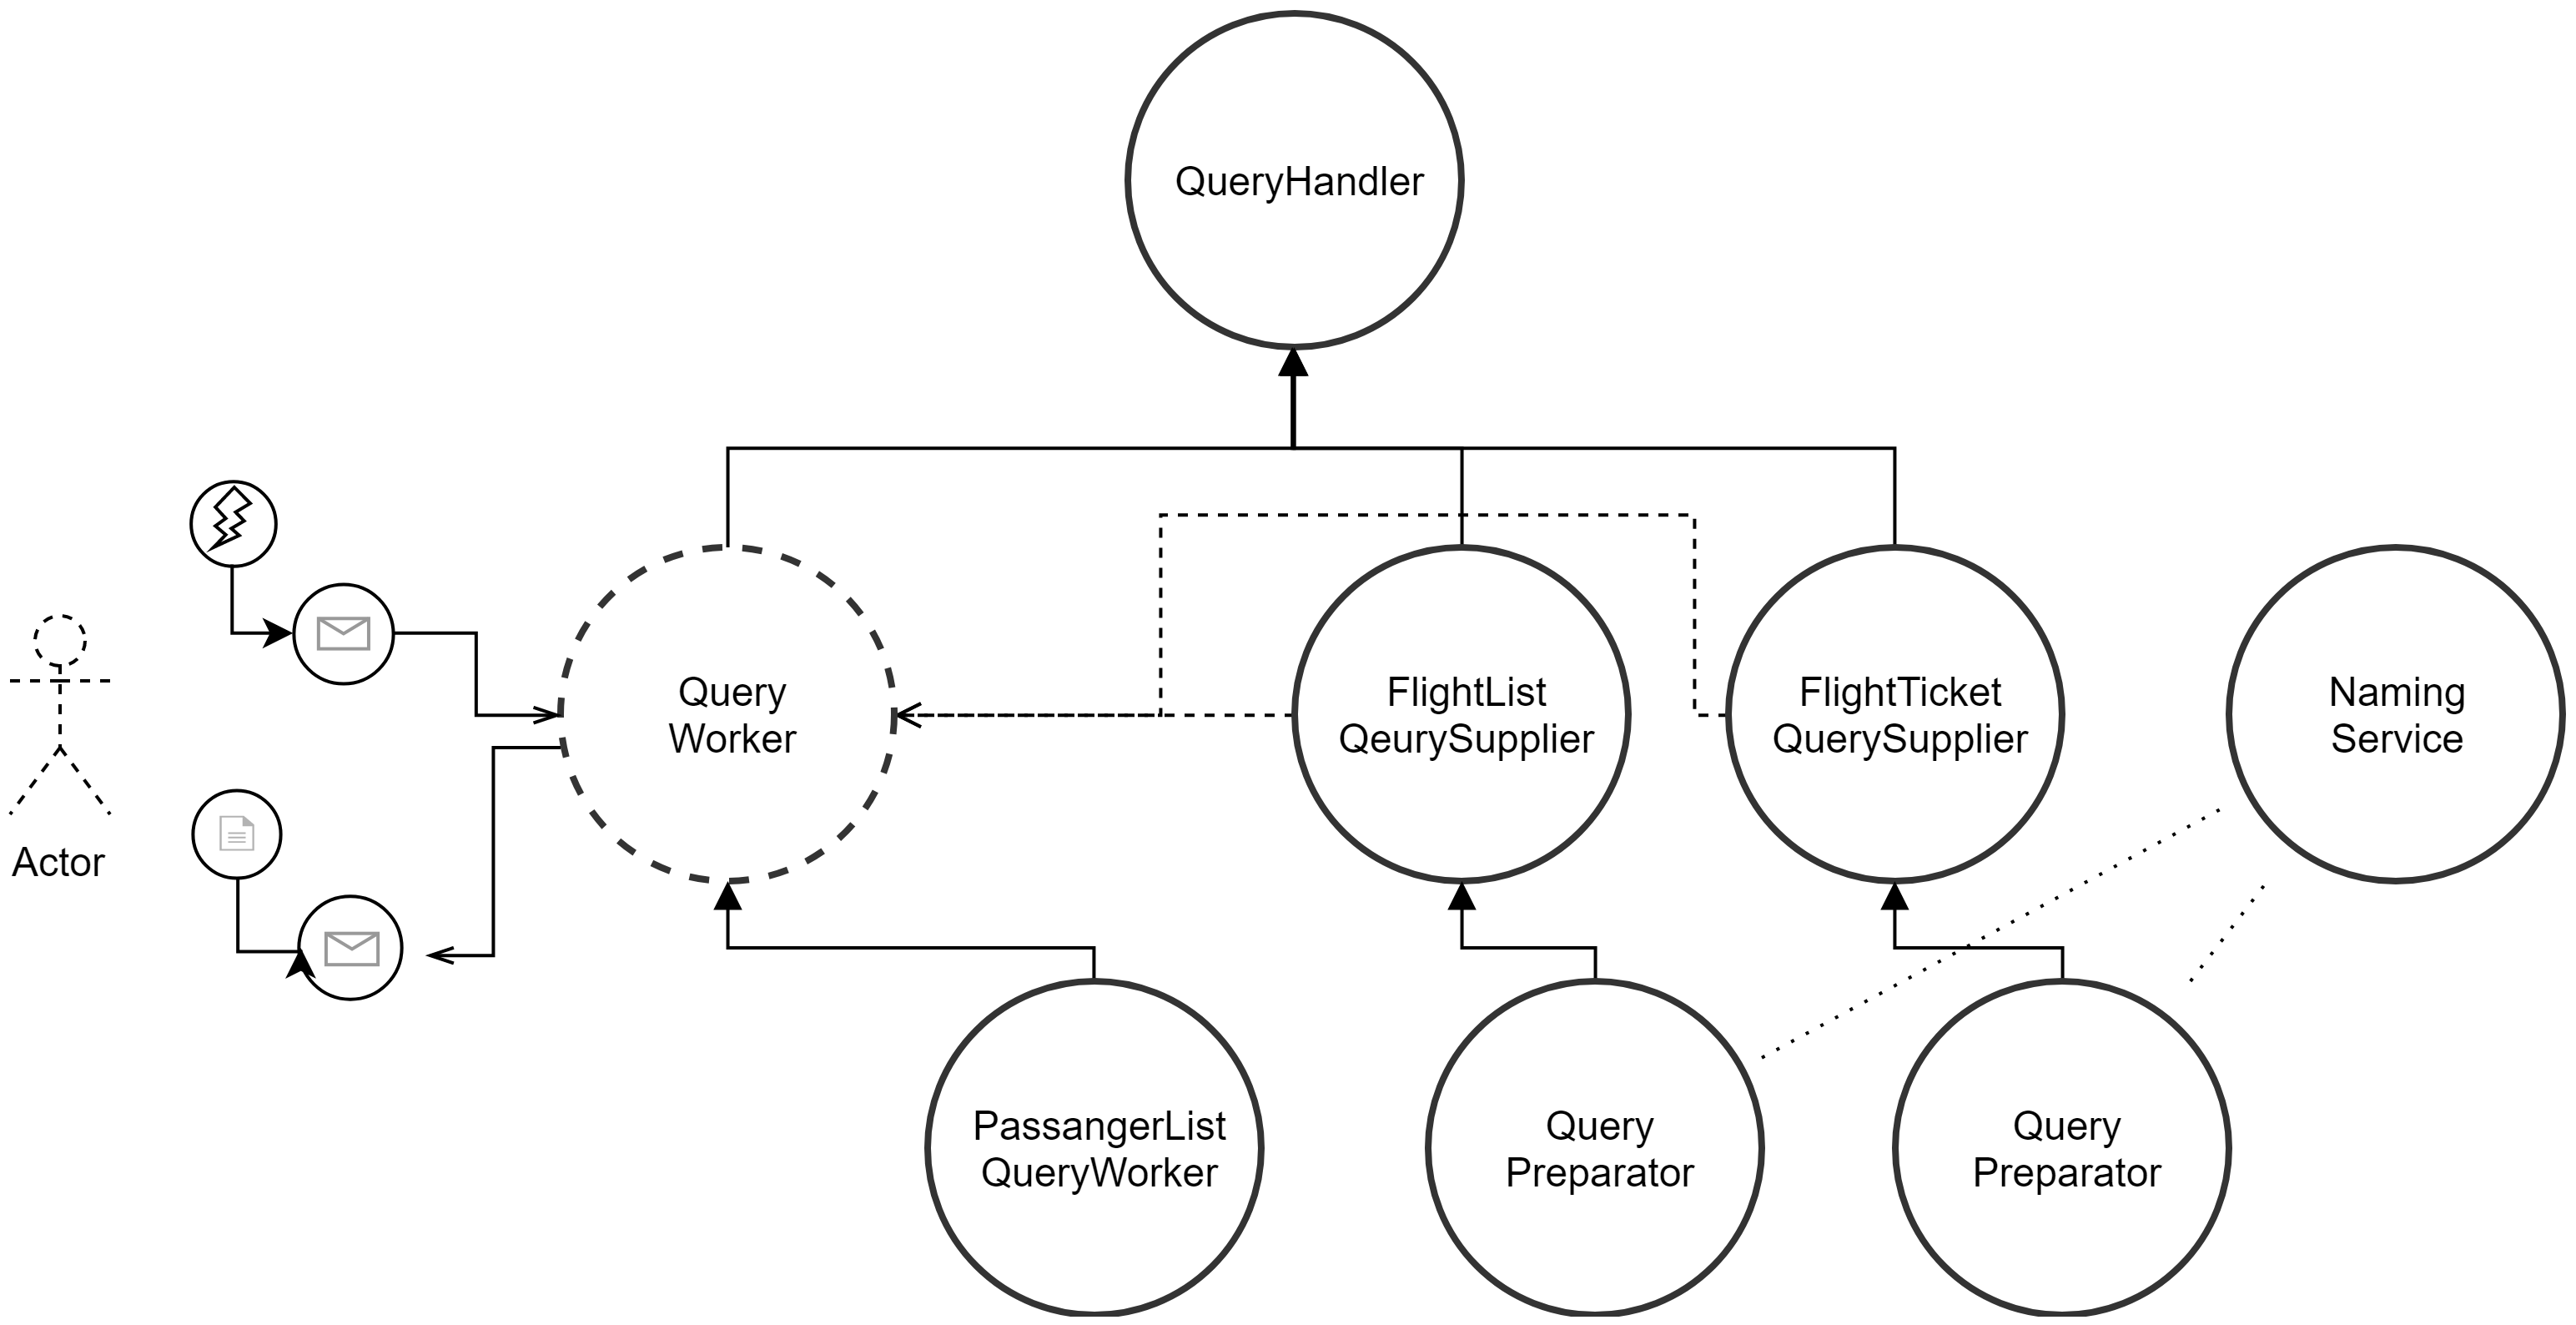
\includegraphics[width=\linewidth]{gfx/implementation/QueringServiceActorModel}
    \caption{Der Aufbau des Actor Systems der Query Komponente von \textit{TyrolSky}.}
    \label{fig:implementation:queryActorModel}
\end{figure} 

\subsection{Command-Service  und Domain-Service}
\label{subsec:implementation:domainService}
\section{Implementierung von Event Sourcing}
\label{subsec:implementation:eventSouring}

\section{Verteilung der Anwendung}
\label{subsec:implementation:ApplicationDistribution}

\subsection{Globale Dienste}
\label{subsec:implementation:singeltons}

\section{Cluster}
\label{subsec:implementation:gossip}
Gossip, 

\subsection{Fixe Dienste}
wtf?
\subsection{Verteilung transaktionaler Daten}
Erklärung von Sharding

\section{Garantierte Nachrichtenübermittelung}

\section{Externe Schnittstellen}
bank api
\section{Testapplikation}

\section{Verwendete Umgebung}
Welche Version, wie genau etc...
